% !TEX root = ../stellar-notes.tex
\chapter{Radiation Transport}


The sun is very opaque.  Were photons able to stream freely, they would exit in $\sim \Rsun/c = 2.0\nsp\second$.  Given the luminosity of the sun, however, we derived that the time  for the sun to radiate away its stored thermal energy is instead millions of years (see eq.~[\ref{e.K-H}]).  As a result, we can regard the sun as a cavity filled with photons with a very slight leakage.  This is the description commonly invoked to describe blackbody radiation, and we expect that in the interior of the sun, the radiation can be described by a photon gas in thermal equilibrium at the ambient temperature.

\section{Description of the Radiation Field}\label{s.radiation-description}

Consider a cavity containing a gas of photons. In general we can describe the mean number of photons in this cavity as
\begin{equation}\label{e.photon-occupation}
 N = \int f(\vp,\vx)\,\dif^{3}x\,\dif^{3}p.
\end{equation}
Here $f$ is a distribution function, as described in Chapter~\ref{ch.equation-of-state}; if we are in thermal equilibrium, $f$ is of course the Bose-Einstein distribution (cf.\ eq.~[\ref{e.boson-dist}]), but our discussion here will be more general.  Consider a small opening on our cavity with area $\dif A$ and unit normal $\unitn$.  The energy incident on this area in a time $\dif t$ having propagation vector along $\unitn$ and propagating into solid angle $\dif\Omega$ (see Fig.~\ref{f.intensity-schematic}) is found by integrating equation~(\ref{e.photon-occupation}) over a volume $\dif^{3}x = c\dif t\,\dif A$,
\[
\dif E = \dif A\,c\dif t\,\left( p^{2}\dif p\,\dif\Omega\right)  h\nu \, f.
\]
Since the photon momentum is $p = h\nu/c$, we have
\begin{equation}\label{e.specific-intensity}
I_{\nu} \equiv \frac{\dif E}{\dif t\,\dif A\,\dif\Omega\,\dif\nu} = \frac{h^{4}\nu^{3}}{c^{2}} f.
\end{equation}
This defines the \emph{specific intensity} $I_{\nu}$.  It is easy to show that in the absence of interactions with matter, $I_{\nu}$ is conserved along a ray (see, e.g., Rybicki \& Lightman).

If the photons are in thermal equilibrium, then $f$ is the Bose-Einstein distribution, $f = (2/h^{3})(\exp[h\nu/\kB T]-1)^{-1}$, and the specific intensity becomes
\begin{equation}\label{e.Bnu}
B_{\nu} \equiv \frac{2 h\nu^{3}}{c^{2}} \left[\exp\left(\frac{h\nu}{\kB T}\right)-1\right]^{-1}.
\end{equation}
Here $B_{\nu}$ is called the \emph{Planck function}.

\begin{marginfigure}
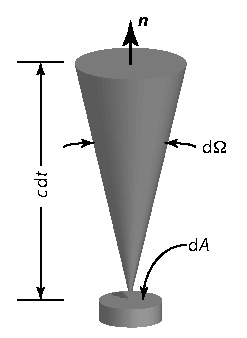
\includegraphics{intensity-schematic}
\caption{\label{f.intensity-schematic}Schematic of a pencil of radiation propagating into an angle $\dif\Omega$.}
\end{marginfigure}

The energy density per frequency $u_{\nu}$ can be defined as $\dif E/(c \dif t\,\dif A\,\dif\nu)$, that is, the energy per unit frequency that is in a cylinder of length $c\,\dif t$ and cross-sectional area $\dif A$; comparing $u_{\nu}$ with the definition of $I_{\nu}$, we see that
\[
u_{\nu} = \frac{1}{c}\int I_{\nu}\,\dif\Omega .
\]
For a blackbody, $I_{\nu}=B_{\nu}$ doesn't depend on angle, and we can integrate over $\dif\Omega$,
\begin{equation}\label{e.radiation-energy-density}
u_{\nu}= \frac{8\pi h\nu^{3}}{c^{3}}\left[\exp\left(\frac{h\nu}{\kB T}\right)-1\right]^{-1}.
\end{equation}
The total energy density can then be found by integrating over all frequencies, giving
\[ u = \left[\frac{8\pi^{5}\kB^{4}}{15 h^{3}c^{3}}\right] T^{4}\equiv aT^{4} \]
in agreement with what we derived from statistical mechanics, \S\ref{s.relativistic-photon-gas}.

The next quantity to define is the \emph{flux} of energy, along direction $\unitk$, per unit time $\dif t$,  per unit area $\dif A$, and per frequency interval $\dif\nu$. We multiply $I_{\nu}$ by a direction vector $\unitk$ and integrate over $\dif\Omega$:
\begin{equation}\label{e.radiation-flux}
\bvec{F}_{\nu} = \int \unitk I_{\nu} \,\dif\Omega.
\end{equation}
Note that $\bvec{F}_{\nu}$ is a vector;  the net flux along a direction \unitn\ is
\[ F_{\nu} = \int I_{\nu}(\unitn\cdot\unitk)\dif\Omega. \]
If we take our polar angle with respect to $\unitk$, then $(\unitn\cdot\unitk)\,\dif\Omega = \cos\theta\,\sin\theta\,\dif\theta\,\dif \phi$; defining the direction cosine $\mu = \cos\theta$, this becomes 
\[ F_{\nu} = \int I_{\nu} (\unitn\cdot\unitk)\,\dif\Omega = \int_{0}^{2\pi} \int_{-1}^{1} I_{\nu}\mu\,\dif\mu\,\dif\phi. \]
Note that if the radiation field is isotropic then $F_{\nu}=0$: there must be some anisotropy in the radiation field to generate a net flux.

For blackbody radiation, if we only integrate over outgoing directions, $0\le \mu\le 1$, as would be the case for thermal radiation emerging from a \emph{hohlraum},
\[ F_{\nu} = \pi B_{\nu}.\]
Integrating this $F_{\nu}$ over all frequencies, we recover the Stefan-Boltzmann formula,
\[ F = \left(\frac{ac}{4}\right) T^{4} \equiv \sigma_{\mathrm{SB}} T^{4}, \]
where $\sigma_{\mathrm{SB}}$ is the Stefan-Boltzmann constant.

Finally, let's look at the momentum flux along direction $\unitj$ being transported along direction \unitk, per unit time $\dif t$, per unit area $\dif A$, and per unit frequency interval $\dif\nu$.  Since for a photon, $E = pc$, we divide the energy flux by $c$.
This is a \emph{tensor},
\begin{equation}\label{e.radiation-pressure-tensor}
\btens{P}_{\nu} = \frac{1}{c}\int \unitj\unitk I_{\nu}\dif\Omega.
\end{equation}
The net (isotropic) momentum flux along a direction \unitn\ is then
\[ P_{\nu} = \frac{1}{c}\int (\unitn\cdot\unitk)(\unitn\cdot\unitk) I_{\nu}\,\dif \Omega = \frac{2\pi}{c}\int_{-1}^{1} I_{\nu}\mu^{2}\,\dif\mu. \]
For blackbody radiation, 
\[ P_{\nu} = \frac{4\pi}{3c} B_{\nu}  = \frac{1}{3}u_{\nu}\]
and we may integrate this over frequency to obtain $P = u/3$, the standard result from thermodynamics.

\section{Some simple estimates}

We argued in the previous section that the solar interior is quite opaque. Naively, we might imagine some radiative transition, e.g. bremsstrahlung, emitting a photon.  The photon speeds away at $c$, but it doesn't get very far before being absorbed or scattered by another particle. A new photon, either due to emission or scattering, will be emitted at some random direction, and the whole process repeats. This is just a description of a \emph{random walk}. 

For some simple estimate, let's assume that the hop is the same for all photons, regardless of frequency or ambient temperature. If the hop length is $\ell$, then we know that the total path length to get from the center to the surface is $\Rsun(\Rsun/\ell)$ and the time for this to occur is $\Rsun^{2}/\ell/c$. What is a good estimate for $\ell$?  Consider a planar electromagnetic wave incident on a collection of scatterers. If these scatterers are uncorrelated, then the probability of scattering is just the number of scatterers times the probability for scattering from a single scatterer.  Define the probability of scattering as
\begin{equation}\label{e.scattering-probability}
\mathcal{P} = N\times\left(\frac{\textrm{energy scattered per unit time by one scatterer}}{\textrm{energy incident per unit time per unit area}}\right)\frac{1}{ \mathcal{A}}
\end{equation}
where $\mathcal{A}$ is the area normal to the propagation direction \unitk\ of the volume containing the $N$ scatterers.  The quantity in parenthesis is just the definition of the cross-section $\sigma$. Furthermore, if we set $\mathcal{P} = 1$, then the total number of scatters is just $N = n\times \mathcal{A}\times \ell$, where $n$ is the number density of scatterers. Thus we define the \emph{mean free path},
\begin{equation}\label{e.mean-free-path}
\ell = \frac{1}{n\sigma}.
\end{equation}
In stellar work, it is more convenient to use mass density rather than number density.  Writing $n = Y\rho/\mb$, where $Y$ is the abundance of scatterers, we have
\[ \ell = \rho^{-1} \left(\frac{\mb}{Y\sigma}\right) \equiv (\rho\kappa)^{-1} \]
where $\kappa$ is the \emph{opacity} and has dimensions $[\kappa]\sim[\cm^{2}\nsp\gram^{-1}]$.

The opacity in the stellar interior is set by a large number of processes (see \S\ref{s.opacity-sources}): Thomson scattering, free-free absorption, atomic absorption, and photoionization.  In general, the cross-section depends on the ambient temperature and density and the frequency of the photon. 
Over the length of a hop $\ell$ the temperature and density will only vary slightly.  As a result, the conditions are nearly isotropic, so we indeed expect the radiation to come into thermal equilibrium with the ambient material.  But the conditions are not perfectly isotropic---otherwise there would be zero net heat flux!  It is the small anisotropy that gives rise to the transport of energy.  Let's imagine a small cube of material, with the size of this cube being $\ell$.  Because we are so very nearly isotropic and in thermal equilibrium, the flux through any one face of this cube must be $(c/6)u$.  Now suppose we have two adjacent cubes, with the common face of the cubes being at $x=0$.  The flux across the face has contributions from photons emitted at $x-\ell$ and $x+\ell$, so the net flux is
\begin{eqnarray}
	F &\approx& \frac{c}{6} u(x-\ell) - \frac{c}{6} u (x+\ell)\nonumber \\
	&\approx& -\frac{1}{3}c\ell\frac{\dif u}{\dif x}.\label{e.rad-diffusion-simple}
\end{eqnarray}
This is a diffusion equation with coefficient $c/(3\rho\kappa)$.  Our derivation is very crude, as it neglects the variation in cross section with the properties of the ambient medium and with the photon frequency.  Nonetheless, this is basically the correct scenario; heat diffuses with a coefficient given by some suitably defined average over all sources of opacity. 

\section{Equation of Transfer}

We're now ready to formalize the crude work in the previous section.
In the absence of interactions with matter, the specific intensity $I_{\nu}$ is conserved along a ray propagating in direction \unitk: $\dif I_{\nu}/\dif s = c^{-1}\partial_{t}I_{\nu} + \unitk\cdot\grad I_{\nu} = 0$. If matter is present, it can do three things to change $I_{\nu}$.
\begin{description}
\item[emit] Matter may spontaneously emit photons and add to the beam: $\dif I_{\nu}/\dif s = \rho\varepsilon_{\nu}/(4\pi)$. Here $\varepsilon_{\nu}$ is the energy spontaneously emitted per unit frequency per unit time per unit mass.  The factor of $4\pi$ is to make this term per steradian.

\item[absorb] Photons have a chance of being absorbed or scattered out of the beam: $\dif I_{\nu}/\dif s = -\rho\kappa_{\nu}I_{\nu}$. Here the right-hand side is the energy removed from the beam along a path $\dif s$ with $\kappa_{\nu} = \kappa_{\nu}^{\mathrm{abs}} + \kappa_{\nu}^{\mathrm{sca}}$ being the total opacity (absorption plus scattering). The dimensions of opacity are clearly $[\kappa_{\nu}] \sim [\cm^{2}/\gram]$. (If we had stimulated emission, this would be a \emph{negative} $\kappa_{\nu}$.)

\item[scatter] Photons may be scattered into the beam from other directions: $\dif I_{\nu}/\dif s = \rho\kappa_{\nu}^{\mathrm{sca}}\phi_{\nu}$. If the scattering is isotropic, then
\begin{equation}\label{e.isosca}
\phi_{\nu} = \frac{1}{4\pi}\int_{0}^{2\pi}\!\!\!\int_{0}^{\pi} I_{\nu}\,\dif\phi\,\sin\theta\,\dif\theta \equiv J_{\nu},
\end{equation}
where $J_{\nu}$ is the mean intensity: the scattering redistributes the energy over all angles.
\end{description}
Putting all these terms together gives us the \emph{equation of transfer},
\begin{equation}\label{e.transfer}
\frac{1}{c}\partial_{t}I_{\nu} + \unitk\cdot\grad I_{\nu} = \rho \frac{\varepsilon_{\nu}}{4\pi} - \rho\kappa_{\nu} I_{\nu} + \rho\kappa_{\nu}^{\mathrm{sca}}\phi_{\nu}
\end{equation}
for the specific intensity $I_{\nu}$.

\subsection{Radiative equilibrium} 
The emissivity $\varepsilon_{\nu}$ and the opacity $\kappa_{\nu}$ describe how the radiation interacts with matter. A condition of steady-state is that the gas not gain or lose energy to the radiation. This requires balancing
\[ \left(\textrm{energy emitted per unit volume}\right) = \rho\int\frac{\varepsilon_{\nu}}{4\pi}\,\dif\nu\,\dif\Omega\] 
with
\[ \left(\textrm{energy absorbed per unit volume}\right) = \rho\int \kappa_{\nu}^{\mathrm{abs}} I_{\nu}\,\dif\nu\,\dif\Omega,\]
or
\begin{equation}\label{e.rad-equil}
\int_{0}^{\infty}\! \left(\frac{\varepsilon_{\nu}}{4\pi} - \kappa_{\nu}^{\mathrm{abs}} J_{\nu}\right)\,\dif\nu = 0.
\end{equation}
Here we assume $\varepsilon_{\nu}$ does not depend on angle. We don't include scattering because it doesn't transfer energy between the radiation and the gas.

Now suppose that the level populations of the matter are in thermal equilibrium and can be described by a temperature $T$.  In that case, detailed balance must hold, so that
\begin{equation}\label{e.detail-balance}
\frac{\varepsilon_{\nu}}{4\pi\kappa_{\nu}^{\mathrm{abs}}} = B_{\nu}(T),
\end{equation}
where $B_{\nu}(T)$ is the Planck function. This defines \emph{local thermodynamic equilibrium (LTE)}. If the radiation field is, in addition, described by a Planck function \emph{at the same temperature} then we would have complete thermodynamic equilibrium.

\subsection{Optical depth}

Consider a ray directed into a medium in steady-state ($\partial_{t}\to 0$).  In the absence of emission ($\varepsilon_{\nu}=0$) or scattering ($\kappa_{\nu}^{\mathrm{sca}}=0$) equation~(\ref{e.transfer}) takes a particularly simple form:
\begin{equation}\label{e.transfer-optical-depth}
\frac{\dif I_{\nu}}{\dif \tau_{\nu}} = -I_{\nu}.
\end{equation}
Here we have set $\unitk\cdot\grad = (\dif/\dif s)$, where $\dif s$ is a infinetesimal along the path of the ray, and further have defined the \emph{optical depth} as
\begin{equation}\label{e.optical-depth-def}
\tau_{\nu} = \int \rho\kappa_{\nu}\,\dif s.
\end{equation}
Note that $\tau_{\nu}$ is dimensionless. Taking $\rho$ and $\kappa_{\nu}$ as given, equation~(\ref{e.transfer-optical-depth}) has a simple solution,
\[ I_{\nu}(\tau_{\nu}) = I_{\nu}(0)\exp\left(-\tau_{\nu}\right). \]
Note that $\rho\kappa=\ell^{-1}$, so equation~(\ref{e.optical-depth-def}) is just $\tau = \int \dif s/\ell$, i.e., it expresses distance by counting the number of mean free pathlengths traversed.

\subsection{Source function}

Having defined the optical depth, we can now add the emissivity $\varepsilon_{\nu}$ and scattering term (henceforth we will assume isotropic scattering) to equation~(\ref{e.transfer-optical-depth}) to obtain
\begin{equation}\label{e.transfer-with-source}
\frac{\dif I_{\nu}}{\dif \tau_{\nu}} = S_{\nu}-I_{\nu},
\end{equation}
where 
\begin{equation}\label{e.source-fcn-def}
S_{\nu} \equiv \frac{1}{\kappa_{\nu}}\left(\frac{\varepsilon_{\nu}}{4\pi} + \kappa_{\nu}^{\mathrm{sca}}J_{\nu}\right)
\end{equation}
is the \emph{source function}. In the absence of scattering, so that $S_{\nu} = \varepsilon_{\nu}/(4\pi\kappa_{\nu})$ is a known function of $\tau_{\nu}$,
we can formally solve equation~(\ref{e.transfer-with-source}):
\[ I_{\nu}(\tau_{\nu}) = I_{\nu}(0)\exp(-\tau_{\nu}) + \int_{0}^{\tau_{\nu}} S_{\nu}(\tau_{\nu}) \exp(t-\tau_{\nu})\,\dif t. \]
In the presence of scattering, $S_{\nu}$ depends on $J_{\nu} = (1/4\pi)\int I_{\nu}\,\dif\Omega$, so that equation~(\ref{e.transfer-with-source}) is an \emph{integro-differential} equation.

\section[Diffusion Approximation]{Diffusion Approximation and the Rosseland Mean Opacity}

At large optical depth, such as deep in a stellar interior, the radiation field is in thermal equilibrium, so that $I_{\nu} = S_{\nu} = B_{\nu}$. To see this, consider the relative scales of terms in the transfer equation.
\begin{center}\begin{tabular}{ccccccccc}
$\displaystyle \frac{1}{c}\frac{\partial I_{\nu}}{\partial t}$ & + &
$\displaystyle  \unitk\cdot\grad I_{\nu}$ & = &
$\displaystyle\rho\frac{\varepsilon_{\nu}}{4\pi} $ & $-$ & 
$\displaystyle \rho\kappa_{\nu} I_{\nu}$ & $+$ &
$\displaystyle \rho\kappa_{\nu}^{\mathrm{sca}} J_{\nu}$\\
I & & II & & III & & IV & & V
\end{tabular}
\end{center}
On the left-hand side, term I scales as $I_{\nu}/(c t_{\odot})$, where $t_{\odot}$ is the evolutionary timescale of the sun ($\Giga\yr$), and term II scales as $I_{\nu}/R_{\odot}$. On the right-hand side, term IV scales at $I_{\nu}/\ell$.  Hence the ratio of terms of term II to term IV is $\ell/R_{\odot}\ll 1$ and that of term I to term IV is $\ell/\Giga\parsec\ll 1$. In addition, stellar properties change negligibly on scales of a mean-free path, so conditions are nearly isotopic over much of the interior and $I_{\nu} = J_{\nu}$. Hence $I_{\nu} = J_{\nu} = S_{\nu}$, and inserting the relation between $\varepsilon_{\nu}$ and $\kappa_{\nu}^{\mathrm{abs}}$ from detailed balance, eq.~(\ref{e.detail-balance}), into equation~(\ref{e.source-fcn-def}) implies that $S_{\nu} = B_{\nu}$.

If the radiation field is perfectly isotropic there is no flux, however, so we must have some small anisotropy. Let's write $I_{\nu}$ as a thermal term plus a correction, 
\[ I_{\nu} = B_{\nu}(T) + I^{(1)}_{\nu}. \]
Substituting this into the steady-state equation of transfer,
\[ \frac{1}{\rho\kappa_{\nu}}\unitk\cdot\grad I_{\nu}  = S_{\nu} - I_{\nu}\]
and setting the term $S_{\nu}-B_{\nu}=0$ on the right-hand side, we obtain
\begin{equation}\label{e.rad-diffusion-1}
I_{\nu}^{(1)} = -\frac{1}{\rho\kappa_{\nu}} \unitk\cdot\grad B_{\nu} = -\frac{1}{\rho\kappa_{\nu}} \frac{\partial B_{\nu}}{\partial T} \unitk\cdot\grad T.
\end{equation}
This is anisotropic: the energy transport is largest in the direction ``down'' the temperature gradient. Let's get the net flux: multiply equation~(\ref{e.rad-diffusion-1}) by $\unitk$ to get the flux; and then take the component along a direction $\unitn$ parallel to $\grad T$; finally replace the two dot products by the angle cosine $\mu$, and integrate over $\dif \Omega = 2\pi \dif\mu$ to obtain
\begin{equation}\label{e.rad-diffusion-2}
\bvec{F}_{\nu} = -\frac{4\pi}{3}\frac{1}{\rho}\left[\frac{1}{\kappa_{\nu}}\frac{\partial B_{\nu}}{\partial T}\right]\grad T.
\end{equation}
The quantity in $[\,]$ deserves a closer look. First, suppose $\kappa_{\nu}$ is independent of frequency. Then equation~(\ref{e.rad-diffusion-2}) means that the energy transport is greatest at the frequency where $\partial B_{\nu}/\partial T$ is maximum, and \emph{not} at the peak of the Planck spectrum. 

\begin{exercisebox}[Weighting by $\partial B_\nu/\partial T$ in radiative diffusion equation]
Explain on physical grounds why the flux for a grey opacity would be greatest at the frequency for which $\partial B_{\nu}/\partial T$, rather than $B_{\nu}$, is maximized.
\end{exercisebox}

Let us define the \emph{Rosseland mean opacity} as
\[ \kappa_{\mathrm{R}} \equiv \left[\frac{\int\,\dif\nu\,\kappa_{\nu}^{-1}(\partial B_{\nu}/\partial T)}{\int \,\dif\nu\, (\partial B_{\nu}/\partial T)}\right]^{-1}. \]
We can use this to integrate equation~(\ref{e.rad-diffusion-2}) to obtain the total radiative flux,
\begin{equation}\label{e.rad-flux}
\bvec{F} = - \frac{4\pi}{3} \frac{1}{\rho\kappa_{\mathrm{R}}} \grad\left[\int\,\dif\nu\,B_{\nu}\right] = - \frac{1}{3} \frac{c}{\rho\kappa_{\mathrm{R}}} \grad aT^{4}.
\end{equation}
This is just our formula for radiation diffusion (eq.~[\ref{e.rad-diffusion-simple}]) that we obtained from physical arguments, but now we have an expression for the effective opacity $\kappa_{\mathrm{R}}$.

\section{Sources of Opacity}\label{s.opacity-sources}

There are several processes that contribute to radiative opacity in stellar interiors.  These are well described in standard texts, so we'll just briefly list them here.

\subsection{Thomson scattering}
Thomson scattering is scattering from non-relativistic electrons when the photon energy is sufficiently low that we can neglect the recoil of the electron.  The cross-section for Thomson scattering derived in Jackson and is 
\begin{equation}\label{e.Thomson-cross-section}
\sigma_{\mathrm{Th}} = \frac{8\pi}{3}\left(\frac{e^{2}}{m_{e}c^{2}}\right)^{2} = 0.665 \times 10^{-24} \nsp\cm^{2}.
\end{equation}
The opacity for Thomson scattering is then
\[ \kappa_{\mathrm{Th}} = \frac{n_{e}\sigma_{\mathrm{Th}}}{\rho} (0.4\nsp\cm^{2}\nsp\gram^{-1}) Y_{e}. \]
The factor of $Y_{e}$ is because the electrons, which are much lighter than nuclei and therefore easier for an incident wave to shake, do the scattering.

\begin{exercisebox}[Photon diffusion time for the sun]
Using Thomson scattering for the dominant opacity, estimate the photon diffusion time for the sun. 
\end{exercisebox}

\subsection{Free-free absorption}
Another important one is free-free absorption. This is the inverse of \emph{bremsstrahlung}, which is radiation emitted when an electron is scattered from an ion (see Figure~\ref{f.scattering}). The procedure for calculating the opacity is to first compute the emissivity and then use detailed balance (eq.~[\ref{e.detail-balance}]) to obtain
\[ \kappa_{\nu}^{\mathrm{ff}} = \frac{\varepsilon_{\nu}}{4\pi B_{\nu}(T)} . \] 
To calculate the emissivity, we start with the derivation of the momentum gained by an electron (eq.~[\ref{e.pperp}]).  The acceleration leads to an emission of radiation; according to Larmor's formula, the power emitted is
\begin{equation}\label{e.larmor}
P(b) = \frac{2}{3}\frac{e^{2}}{c^{3}} |\bvec{\dot{v}}|^{2} = \frac{2}{3}\frac{Z^{2}e^{6}}{m_{e}^{2}c^{3}b^{4}}.
\end{equation}
The radiation is distributed over a broad range of frequencies up to a cutoff $\nu_{\max}\sim v/b$. Integrating over a range of impact parameters and then over the distribution of electron velocities gives the emissivity, which is (restoring all of the numerical factors)
\begin{equation}\label{e.free-free-w}
\rho \varepsilon_{\nu} = 4\pi\left(\frac{2\pi}{3}\right)^{1/2}Z^{2}n_{I}n_{e} \hbar c^{2}  \alpha \sigma_{\mathrm{Th}} \left(\frac{m_{e}}{\kB T}\right)^{1/2}\,\exp\left(-\frac{h\nu}{\kB T}\right) \bar{g}_{\mathrm{ff}}.
\end{equation}
The velocity-averaged Gaunt factor $\bar{g}_{\mathrm{ff}}$ contains most of the details about the integration. The factor of $T^{-1/2}$ is because there is a factor of $v^{-1}$ that appears in the integration (the collision time is $\sim b/v$).  

Applying detailed balance, equation~(\ref{e.detail-balance}), gives the opacity as a function of frequency,
\begin{equation}\label{e.free-free-opacity}
\kappa^{\mathrm{ff}}_{\nu} = \pi\left(\frac{2\pi}{3}\right)^{1/2}Z^{2}\frac{n_{I}n_{e}}{\rho}c^{3}\alpha \sigma_{\mathrm{Th}} \left(\frac{m_{e}c^{2}}{\kB T}\right)^{1/2} \nu^{-3} \left[ 1- \exp\left(-\frac{h\nu}{\kB T}\right)  \right] \bar{g}_{\mathrm{ff}}
\end{equation}
Notice that $n_{I}n_{e}/\rho = \rho/(\mb^{2}\mu_{I}\mu_{e})$, so that the opacity scales with density.  Further, note that when taking the Rosseland mean over all frequencies, the factor of $\nu^{-3}$ introduces a factor of $T^{-3}$, so that $\langle\kappa^{\mathrm{ff}}_{\nu}\rangle \propto \rho T^{-7/2}$.

\begin{exercisebox}[Relative importance of free-free and Thomson scattering]
In terms of central density and temperature, under what conditions is free-free opacity more important than Thomson scattering?  For what mass range of stars is free-free opacity dominant in the core? What about for Thomson scattering?
\end{exercisebox}

\subsection{Bound-free and bound-bound absorption; Kramer's opacity}
Bound-free and bound-bound transitions have a cross-section with a frequency dependence (at photon energies above threshold) of $\nu^{-3}$ as well; therefore their Rosseland averages also scale as $\rho T^{-7/2}$.  An opacities with this form is known as {Kramer's opacity}, $\kappa = \kappa_{0}\rho T^{-3.5}$.  For conditions in the solar center, a good approximation is
\begin{eqnarray}
\lefteqn{\kappa \approx 0.012\nsp\cm^{2}\usp\gram^{-1}\left(\frac{\rho}{1\nsp\grampercc}\right) \left(\frac{T}{10^{7}\nsp\K}\right)^{-7/2}} \nonumber\\
&& \times\left[\left(1+X_{\mathrm{H}}\right)\left(X_{\mathrm{H}} + X_{\mathrm{He}} + \sum_{Z>2}\frac{X_{i}Z_{i}^{2}}{A_{i}}\right)\right].
\label{e.kramers-opacity}
\end{eqnarray}
The expression in $[\,]$ is just an approximation for $Y_{e}\langle Z^{2}\rangle$ at solar composition.

\begin{exercisebox}[Rosseland mean for different opacity channels]
 Suppose both free-free absorption ($\kappa^{\mathrm{ff}}_{\nu}$) and Thomson scattering ($\kappa^{\mathrm{Th}}_{\nu}$) contribute to the opacity. Denote by $\langle\,\rangle$ the Rosseland averaging of an opacity.  Does $\langle \kappa^{\mathrm{ff}}_{\nu} + \kappa^{\mathrm{Th}}_{\nu}\rangle = \langle\kappa^{\mathrm{ff}}_{\nu}\rangle+\langle\kappa^{\mathrm{Th}}_{\nu}\rangle$? 

Now suppose that $\kappa^{\mathrm{ff}}_{\nu}$ is due to free-free absorption on two different ion species (denoted below by subscripts ``1'' and ``2'') with different charge number $Z$.  In this case does $\langle \kappa^{\mathrm{ff}}_{\nu,1} + \kappa^{\mathrm{ff}}_{\nu,2}\rangle = \langle\kappa^{\mathrm{ff}}_{\nu,1}\rangle+\langle\kappa^{\mathrm{ff}}_{\nu,2}\rangle$?
\end{exercisebox}

%\subsection{H- Opacity}

\section{Eddington Standard Model}\label{s.LE-Eddington-Standard-Model}

Polytropes with index $n=3/2$ correspond to fully convective stars ($P \propto \rho^{5/3}$, the relation for an adiabat) or for white dwarfs (non-relativistic, degenerate equation of state). Another interesting case, for historical reasons, is the \emph{Eddington Standard Model}, which is a fair approximation to main-sequence stars with $M \gtrsim M_{\sun}$.  Suppose we write the equation of state as the sum of ideal gas and radiation pressure,
\begin{equation}\label{e.eos-with-rad}
 P  = \frac{\rho\kB T}{\mu \mb} + \frac{1}{3}a T^{4}.
\end{equation}
Now make the \emph{ansatz} that
\begin{equation}\label{e.beta-def}
\frac{P_{\mathrm{rad}}}{P} = \frac{aT^{4}}{3P} = 1-\beta = \mathrm{const.},
\end{equation}
that is, the radiation pressure is a fixed fraction of the total pressure everywhere.
Solving for $T$ in terms of $P$ and $\beta$,
\[ T = \left[\frac{3(1-\beta) P}{a}\right]^{1/4}, \]
and inserting this into equation~(\ref{e.eos-with-rad}) gives us a simple EOS,
\begin{equation}\label{e.beta-eos}
P = \left[\left(\frac{\kB}{\mu\mb}\right)^{4}\frac{3}{a}\right]^{1/3}\left[\frac{1-\beta}{\beta^{4}}\right]^{1/3} \rho^{4/3}.
\end{equation}
This is the equation for a polytrope of index 3.

\begin{exercisebox}[Radiation $\beta$ in the Eddington standard model]
Derive an expression for $\beta$ in terms of the mass of the star for the Eddington Standard Model.
\end{exercisebox}

Why is it at all reasonable to take $\beta$ as being constant? To explore this, go back to the equation for radiative diffusion
\[ F(r) = -\frac{1}{3}\frac{c}{\rho\kappa}\frac{\dif aT^{4}}{\dif r}. \]
Write the flux as $F(r) = L(r)/(4\pi r^{2})$, and since pressure decreases monotonically with radius, write
\[ 
\frac{\dif aT^{4}}{\dif r} = \frac{\dif aT^{4}}{\dif P}\frac{\dif P}{\dif r} = -\rho\frac{Gm(r)}{r^{2}}\frac{\dif aT^{4}}{\dif P}. 
\]
The equation of radiation transport then becomes
\[ L(r) = \frac{4\pi Gm(r) c}{\kappa(r)} \frac{\dif P_{\mathrm{rad}}}{\dif P}. \]
Dividing both sides by $L\cdot M/\kappa_{\mathrm{Th}}$ and rearranging terms,
\begin{equation}\label{e.Prad-P}
 \frac{\dif P_{\mathrm{rad}}}{\dif P} = \left[\frac{L\kappa_{\mathrm{Th}}}{4\pi GMc}\right]\left(\frac{\kappa(r)}{\kappa_{\mathrm{Th}}}\frac{L(r)}{L}\frac{M}{m(r)}\right).
\end{equation}
Here $L$ is the total luminosity of the star and $M$ is the total mass.  The term in $[\,]$ is a constant (the Thomson opacity $\kappa_{\mathrm{Th}}$ doesn't depend on density or temperature) and we define the \emph{Eddington luminosity} as $L_{\mathrm{Edd}}=4\pi GM c/\kappa_{\mathrm{Th}}$.  For the sun, $L_{\mathrm{Edd}} = 1.5\ee{38}\nsp\ergs\usp\second^{-1} = 3.8\ee{4}\nsp L_{\sun}$.  For the term $(\,)$ on the right-hand side, note the $L(r)/m(r)$ is basically the average energy generation rate interior to a radius $r$.  Since nuclear reactions are temperature sensitive, the heating is concentrated toward the stellar center and $L(r)/m(r)$ decreases with radius. For stars like the sun, free-free opacity is dominant, and since the free-free Rosseland opacity goes as $T^{-3.5}$, $\kappa(r)$ increases with radius.  Thus, if the energy generation rate is not too temperature dependent (the reaction $\pt + \pt \to \hydrogen[2]$ goes roughly as $T^{4.5}$ at $T=10^{7}\nsp\K$), then the term in $(\,)$  does not vary strongly with radius, and $\dif P_{\mathrm{rad}}/\dif P$ is indeed roughly constant. 


\begin{exercisebox}[Dependence of luminosity on stellar mass]
You are now in a position to understand why the luminosity depends strongly on the mass. Cast the flux equation (eq.~[\ref{e.rad-flux}]) into dimensionless form.  Assume the opacity has the functional form $\kappa = \kappa_{0} \rho^{a} T^{-b}$, and scale $\rho$ and $T$ in terms of $M$ and $R$. 

\begin{enumerate}
\item You should be able to find a characteristic scale for the luminosity which depends on the stellar mass $M$ and radius $R$, as well as on the exponents $a$ and $b$. Regard $\kappa_{0}$ as a fitting constant, and adjust it so that you get an expression in the form
\[
	\frac{L}{\Lsun} = \left(\frac{M}{\Msun}\right)^{\alpha} \left(\frac{R}{\Rsun}\right)^{\beta}.
\]

\item If the opacity is dominated by Thomson scattering, what are $\alpha$ and $\beta$?  What about if the opacity is Kramer's (eq.~[\ref{e.kramers-opacity}])?
\end{enumerate}
\end{exercisebox}


% !TEX root = ../stellar-notes.tex

\DefineShortVerb{\|}

\section*{\raisebox{-0.015ex}{\includegraphics[height=1.4ex]{mesa_logo2}} Radiation pressure and the Eddington luminosity for massive stars}

Construct zero-age main-sequence (ZAMS) stars of masses $\val{1.0}{\Msun}$, $\val{3.0}{\Msun}$, $\val{10.0}{\Msun}$, and $\val{30.0}{\Msun}$. You will find the template for the project in  the folder |radiation/beta-eddington|. 

\begin{enumerate}
\item For each star, plot $\beta\equiv \Pgas/P$ as a function of Lagrangian mass coordinate $m$. Is $\beta$ roughly constant, i.e., independent of $m$? For each ZAMS model, assign a ``typical'' value of $\beta$ and plot this $\beta$ as a function of the total stellar mass $M$.  How well does $\beta(M)$ agree with what you derived in exercise~\ref{p.radiation-beta}?

\item For each star, plot $\Lrad/\Ledd$ as a function of $m$.
\end{enumerate}
The template project files are set up to load a file `|inlist_radn_vars|', which you will write.  The file should contain a customized version of `|Profile_Panels1|' that displays the $\beta$ and $\Lrad/\Ledd$. Note that the values of $\beta$ and $\Lrad/\Ledd$ are not output by default, so you will need to add them to the list of columns in the `profile' data files, as we did in previous exercises.

Finally, you may notice that things get interesting near the surface of the star, especially for the more massive stars.  Change the independent variable from `|mass|' to `|logxq|' and redo the plots. (You may need to adjust the minimum value of the x-axis and reverse the direction of the x-axis.) Comment on the results.

\UndefineShortVerb{\|}

